
\subsection{Сложное движение точки и твёрдого тела}

\subsubsection*{2.15}

% \begin{wrapfigure}{r}{0.25\textwidth}
%   \begin{center}
%         \vspace{-20 mm}
%         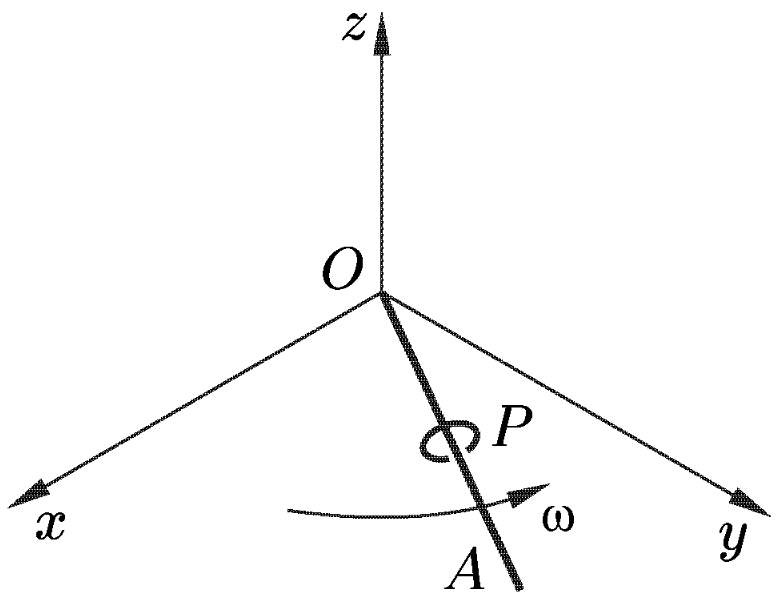
\includegraphics[width=0.8\linewidth]{img/2_15.png}
%   \end{center}
% \end{wrapfigure}

Для началача найдём, что
$$
    \left.\begin{aligned}
        \vv{OP} = \vc{r}_p^r &= \vc{a} \cdot (1 + \sin \omega_0 t) \\
        \vc{v}_p^r &= \vc{a} \cdot \omega_0 \cos \omega_0 t \\
        \vc{\mathrm{w}}_p^r &= -\vc{a} \cdot \omega_0^2 \sin \omega_0 t
    \end{aligned}\right\} \text{ в СО стержня, где }
    \vc{a} = a \begin{pmatrix}
        \sin \omega t \\
        \cos \omega t \\
        0
    \end{pmatrix}.
$$

Запишем абсолютную скорость $\vc{v}_p^a$ точки $P$,
$$
    \vc{v}_p^a = \vc{\omega} \times \vc{r}_p^r + \vc{v}_p^r =
    a \omega (1 + \sin \omega_0 t) \begin{pmatrix}
        -\cos \omega t \\
        \sin \omega t \\
        0 
    \end{pmatrix}
    + a \omega_0 \cos \omega_0 t \begin{pmatrix}
        \sin \omega t \\
        \cos \omega t \\
        0
    \end{pmatrix}
$$
Тогда норма $\vc{\|v}_p^a\|$ такая, что
$$
    \|\vc{v}_p^a\|^2 = a^2 \left(
        \omega^2 (1+\sin \omega_0 t) +
        \omega_0^2 \cos \omega_0 t
    \right).
$$
Запишем абсолютное ускорение $\vc{\mathrm{w}}_p^a$ точки $P$,
$$
    \vc{\mathrm{w}}_p^a = - \omega^2 \vc{r}_p^r + 0 + \vc{\omega} \times  \vc{\omega} \times \vc{r}_p^r + 2 \vc{\omega} \times \vc{v}_p^r + \vc{\mathrm{w}}_p^r
    =
    \left(a (\omega^2 + \omega_0^2) \sin \omega_0 t + \omega^2\right) \begin{pmatrix}
        - \sin \omega t \\
        - \cos \omega t \\
        0
    \end{pmatrix}
    +
    2 a \omega \omega_0 \cos \omega_0 t
    \begin{pmatrix}
        - \cos \omega t \\
        \sin \omega t \\
        0
    \end{pmatrix}.
$$
Тогда норма $ \|\vc{\mathrm{w}}_p^a\|^2 $ такая, что
$$
    \|\vc{\mathrm{w}}_p^a\|^2 = \left(
        a (\omega^2 + \omega_0^2) \sin \omega_0 t + \omega^2
    \right)^2 +
    4 a^2 \omega^2 \omega_0^2 \cos^2 \omega_0 t.
$$
\begin{figure}[h]
    \centering
    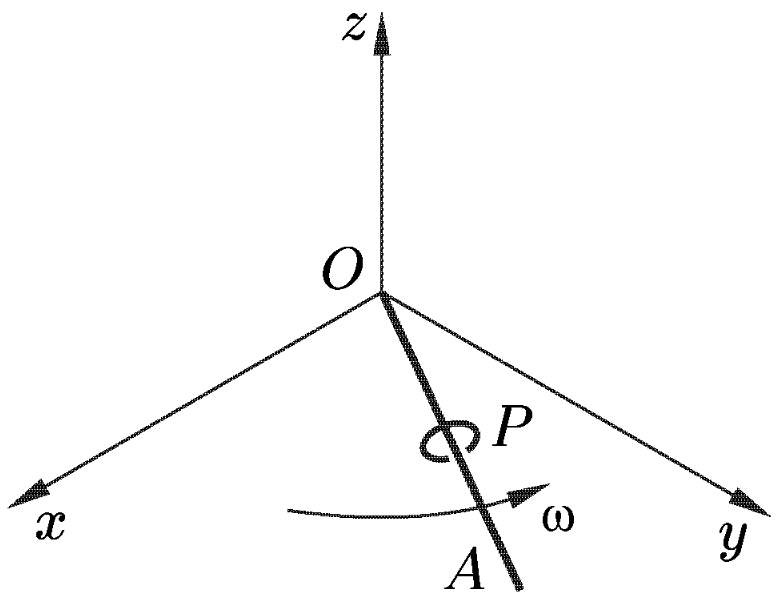
\includegraphics[width=0.24\textwidth]{img/2_15.png}
    \hspace{1cm} 
    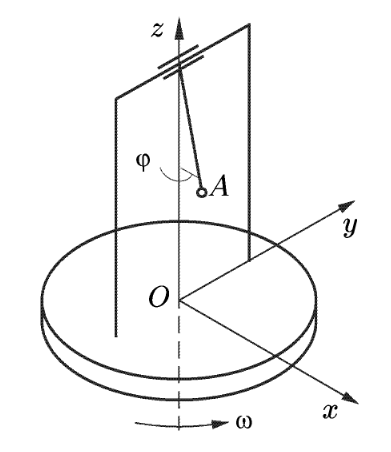
\includegraphics[width=0.2\textwidth]{img/2_19.png}
    \hspace{1cm} 
    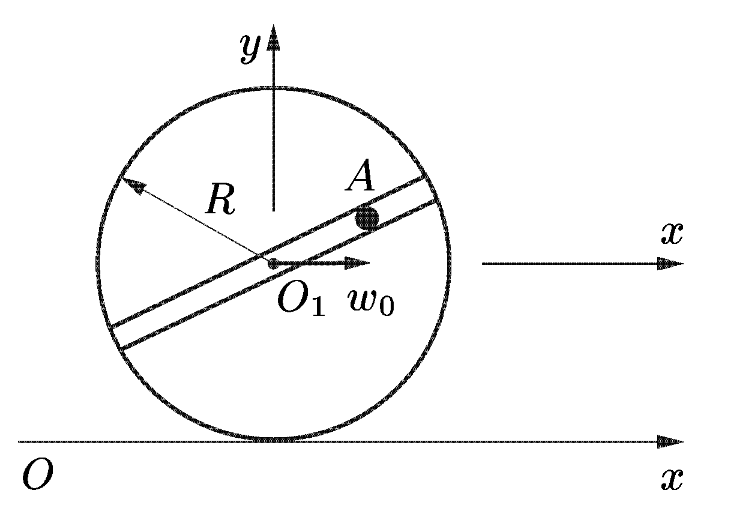
\includegraphics[width=0.3\textwidth]{img/2_35.png}
    \caption{Рисунки к задачам 2.15, 2.19 и 2.35.}
    %\label{fig:}
\end{figure}

\subsubsection*{2.19}

Для начала найдём и выразим все интересные нам векторы:
$$
    \left.\begin{aligned}
        \varphi         &= \varphi_0 \sin \omega_0 t            \\
        \dot{\varphi}   &= \varphi_0 \omega_0 \cos \omega_0 t   \\
        \ddot{\varphi}  &= - \varphi_0 \omega_0^2 \sin \omega_0 t \\
    \end{aligned}\right\},
    \vc{\mathrm{w}}_0 = - \begin{pmatrix}
        \omega^2 r \sin \varphi \\ 0 \\ 0
    \end{pmatrix},
    \vc{\omega}_m = \begin{pmatrix}
        0 \\ - \dot{\varphi} \\ 0
    \end{pmatrix},
    \vv{BA} = r \begin{pmatrix}
        \sin \varphi \\ 0 \\ - \cos \varphi
    \end{pmatrix},
    \vc{\varepsilon}^r = \begin{pmatrix}
        0 \\ -\ddot{\varphi} \\ 0
    \end{pmatrix},
$$

% \begin{wrapfigure}{r}{0.25\textwidth}
%   \begin{center}
%         \vspace{-5 mm}
%         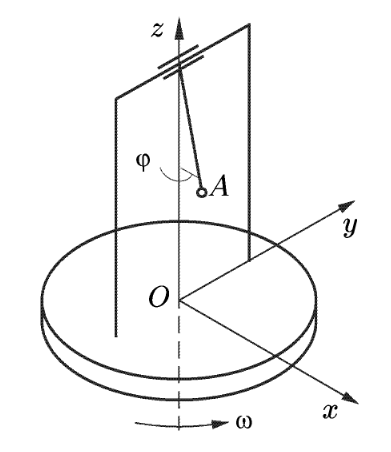
\includegraphics[width=0.8\linewidth]{img/2_19.png}
%   \end{center}
% \end{wrapfigure}

\noindent
где $\vc{\omega}_m$ -- угловая скорость $\vv{AB}$ относительно конструкции.

Во-первых, скорость $\vc{v}_A^a$ такая, что
$$
    \vc{v}_A^a = \vc{v}^e + \vc{v}^r = \vc{\omega} \times \vv{OA} + \vc{\omega}_m \times \vv{BA} =
    r \begin{pmatrix}
        \dot{\varphi} \cos \varphi \\ \omega \sin \varphi \\ \dot{\varphi} \sin \varphi,
    \end{pmatrix}
$$
а норма $\|\vc{v}_A^a\|$ в точке $t=t_0 = \pi / 2 \omega_0$ такая, что
$$
    \|\vc{v}_A^a\|^2 = r^2 \left(\dot{\varphi} + \omega^2 \sin^2 \varphi \right)
    \hspace{0.5cm} \Rightarrow \hspace{0.5cm} 
    \|\vc{v}_A^a\|^2 \bigg|_{t=t_0} = r^2 \omega^2 \sin^2 \varphi_0.
$$
Во-вторых, ускорение $\vc{\mathrm{w}}_A^a$ такое, что
$$
    \vc{\mathrm{w}}_A^a = \vc{\mathrm{w}}_0 + 0 + \vc{\omega} \times \vc{\omega} \times \vv{BA} + 2 \vc{\omega} \times \left(
        \vc{\omega}_m \times \vv{BA}
    \right) + \vc{\mathrm{w}}^r.
$$
Подставляя значения для $t=t_0$, получим, что
$$
    \vc{\mathrm{w}}_A^a =
    -r
    \begin{pmatrix}
        \omega^2 \sin \varphi_0 + \varphi_0 \omega_0^2 \cos \varphi_0 \\
        0\\
        \varphi_0 \omega_0^2 \sin \varphi_0
    \end{pmatrix}.
$$
Соответсвенно, норма ускорения точки $A$
\begin{align*}
        \|\vc{\mathrm{w}}_A^a\|^2 &= r^2(
        \omega^4 \sin^2 \varphi_0 + \omega^2 \omega_0^2 \varphi_0 \sin^2 \varphi_0 +
        \varphi_0^2 \omega_0^4 \cos^2 \varphi_0 + \varphi_0^2 \omega_0^4 \sin^2 \varphi_0
        ) = \\
        &=r^2(\omega^4 \sin^2 \varphi_0 + \omega^2 \omega_0^2 \varphi_0 \sin^2 \varphi_0
                + \varphi_0^2 \omega_0^4).
\end{align*}

%%%%%%%%%%%%%%%%%%%%%%%%%%%%%%%%%%%%%%%%%%%%%%%%%%%%%%%%%%%%%%%%%%%%%%%%%%%%%%%%%%
\subsubsection*{2.35}
%%%%%%%%%%%%%%%%%%%%%%%%%%%%%%%%%%%%%%%%%%%%%%%%%%%%%%%%%%%%%%%%%%%%%%%%%%%%%%%%%%

Снова предварительно запишем необходимые нам величины,
$$
\left.\begin{aligned}
    \vv{O_1A} = \vc{r}_A^r &= \vc{a} \sin \omega t, \\
    \vc{v}_A^r &= \vc{a} \omega \cos \omega t, \\
    \vc{\mathrm{w}}_A^r &= - \vc{a} \omega^2 \sin \omega t\\
\end{aligned}\right\}, \hspace{0.4cm} 
\vc{a} = a \begin{pmatrix}
    \cos \varphi \\ \sin \varphi \\ 0
\end{pmatrix}, \hspace{0.4cm} 
\varphi = - \frac{\vc{\mathrm{w}}_0 t^2}{2R},\hspace{0.4cm} 
\vc{v}_0 = \vc{\Omega} R = \vc{\mathrm{w}}_0 t,\hspace{0.4cm} 
\vc{\varepsilon} = \begin{pmatrix}
    0 \\ 0 \\ \mathrm{w}_0 / R
\end{pmatrix}.
$$
где $\varphi(t)$ и $\vc{\Omega}(t)$ мы знаем из условия $\vc{\mathrm{w}}_0 = \const$.

Скорость $\vc{v}_A^a$ такая, что
$$
    \vc{v}_A^a = \vc{v}_0 + \vc{\Omega} \times  \vc{r}_A^r 
    + \vc{v}_A^r 
    \hspace{0.5cm} \Rightarrow \hspace{0.5cm} 
    \left\{\begin{aligned}
        v_x &= \mathrm{w_0} t\left(
            R + a \sin \varphi \sin \omega t
        \right) / R + a \omega \cos \varphi \cos \omega t \\
        v_y &= a \omega \sin \varphi \cos \omega t - 
        \mathrm{w}_0 t a \cos \varphi \sin \omega t / R\\
        v_z &= 0 \\
    \end{aligned}\right.
$$
а норма 
$$
    \|\vc{v}_A^a\|^2 = \frac{\mathrm{w_0}^2 t^2}{R^2}  a^2 \sin^2 \omega t +
    a^2 \omega^2 \cos^2 \omega t +
    \mathrm{w}_0^2 t^2 +
    2 \frac{\mathrm{w_0}t}{R}a \left(
        \mathrm{w}_0 t \sin \varphi \sin \omega t + R \omega \cos \varphi \cos \omega t
    \right).
$$
или, преобразуя, получим, что
$$
    \|\vc{v}_A^a\|^2 = 
    \left(
        \frac{\mathrm{w}_0 t}{R} a \sin \omega t  \mathrm{w}_0 t \sin \varphi 
    \right)^2 + \left( \vphantom{\frac{1}{2}}
        a \omega \cos \omega t + w_0 t \cos \varphi
    \right)^2.
$$

Ускорение $\vc{\mathrm{w}}_A^a$ такое, что
$$
    \vc{\mathrm{w}}_A^a = 
    \vc{\mathrm{w}}_0 + \vc{\varepsilon} \times \vc{r}_A^r +
    \Omega \times \Omega \times \vc{r}_A^r +
    2 \vc{\Omega} \times \vc{v}_A^r + \vc{\mathrm{w}}^r_A.
$$
Подставляя значения, получим
$$
    \vc{\mathrm{w}}^c = \frac{1}{R} 
    \left(\begin{matrix}2 \omega a t \mathrm{w}_0 \sin{\left(\varphi \right)} \cos{\left(\omega t \right)}\\- 2 \omega a t \mathrm{w}_0 \cos{\left(\varphi \right)} \cos{\left(\omega t \right)}\\0\end{matrix}\right), \hspace{0.7cm} 
    % 
    \vc{\mathrm{w}}^e = \frac{1}{R^2} 
     \left(\begin{matrix}\mathrm{w}_0 \left(R^{2} + R a \sin{\left(\varphi \right)} \sin{\left(\omega t \right)} - a t^{2} \mathrm{w}_0 \sin{\left(\omega t \right)} \cos{\left(\varphi \right)}\right)\\- a \mathrm{w}_0 \left(R \cos{\left(\varphi \right)} + t^{2} \mathrm{w}_0 \sin{\left(\varphi \right)}\right) \sin{\left(\omega t \right)}\\0\end{matrix}\right).
$$
Суммруя, получим, что
$$
    \left\{\begin{aligned}
        \left(\vc{\mathrm{w}}_A^a\right)_x &= 
        \frac{1}{R^2} \left(
            R^{2} \left(- \omega^{2} a \sin{\left(\omega t \right)} \cos{\left(\varphi \right)} + \mathrm{w}_0\right) + R a \mathrm{w}_0 \left(2 \omega t \cos{\left(\omega t \right)} + \sin{\left(\omega t \right)}\right) \sin{\left(\varphi \right)} - a t^{2} \mathrm{w}_0^{2} \sin{\left(\omega t \right)} \cos{\left(\varphi \right)}
        \right) \\
    \left(\vc{\mathrm{w}}_A^a\right)_y &= 
    \frac{1}{R^2} \left(
        - a \left(R^{2} \omega^{2} \sin{\left(\varphi \right)} \sin{\left(\omega t \right)} + R \mathrm{w}_0 \left(2 \omega t \cos{\left(\omega t \right)} + \sin{\left(\omega t \right)}\right) \cos{\left(\varphi \right)} + t^{2} \mathrm{w}_0^{2} \sin{\left(\varphi \right)} \sin{\left(\omega t \right)}\right)
    \right) \\
    \left(\vc{\mathrm{w}}_A^a\right)_z &= 0.
    \end{aligned}\right.
$$



%%%%%%%%%%%%%%%%%%%%%%%%%%%%%%%%%%%%%%%%%%%%%%%%%%%%%%%%%%%%%%%%%%%%%%%%%%%%%%%%%%
\subsubsection*{4.14 и 4.15*}
%%%%%%%%%%%%%%%%%%%%%%%%%%%%%%%%%%%%%%%%%%%%%%%%%%%%%%%%%%%%%%%%%%%%%%%%%%%%%%%%%%

Сделаем задачу чуть менее абстрактной. Представим кольцевую железную дорогу, плоскость которой нормальна к $\vc{\omega}_1$. Наш агент  \textnumero 1 сидит в вагоне поезда и на столе, поверхность которого нормальна к $\vc{\omega}_2$, запускает игрушечную кольцевую жилезную дорогу с игрушечным агентом  \textnumero 2 в вагоне поезда. Агент  \textnumero 2 запускает поезд на столе, поверхность которого нормальна к $\vc{\omega}_3$ ...

Найдём $\vc{\varepsilon}_{\text{\textnumero} 2}$ -- угловое ускорение агента \textnumero 2. По словам \textnumero 1, угловое ускорение равно $\vc{\omega}_{\text{\textnumero 2}} = \vc{\omega}_2$, тогда
$$
    \vc{\varepsilon}_{\text{\textnumero} 2} = \underbrace{\vc{\varepsilon}_1}_{\vc{\varepsilon}^e} + \frac{d}{dt} \vc{\omega}_2 = 0 + 
    \frac{\vc{\omega}_2}{\omega_2} \dot{\omega}_2
    + 
    \vc{\omega}_1 \times \vc{\omega}_2.
$$
А теперь найдём $\vc{\varepsilon}_3$. С точки зрения \textnumero 2 $\vc{\omega}_{\text{\textnumero 3}} = \vc{\omega}_3$. Мы знаем, что $\vc{\omega}_{\text{\textnumero 2}} = \vc{\omega}_1 + \vc{\omega}_2$, и знаем $\vc{\varepsilon}_{\text{\textnumero} 2}$, тогда
$$
    \vc{\varepsilon}_{\text{\textnumero} 3} = \vc{\varepsilon}_2 + \frac{d}{dt} \vc{\omega}_3 = 
    \left(\frac{\vc{\omega}_2}{\omega_2} \dot{\omega}_2 + \vc{\omega}_1 \times \vc{\omega}_2\right)
    + 
    \frac{\vc{\omega}_3}{\omega_3} \dot{\omega}_3
    + 
    (\vc{\omega}_1 + \vc{\omega}_2) \times \vc{\omega}_3.
$$
И так далее мы можем продолжать добавлять вектора $\vc{\omega}_i$ к движению тела, в силу $\vc{\omega}^a = \vc{\omega}^e + \vc{\omega}^r$, при чём мы получим слагаемые вида векторного произведение всех упорядоченных пар $\vc{\omega}_j$ и $\vc{\omega}_k$, плюс сумма $\vc{\varepsilon}^r_i$.
$$
    \vc{\varepsilon}_{\text{\textnumero} N} = \vc{\varepsilon}_{\text{\textnumero} (N-1)} + 
    \frac{\vc{\omega}_N}{\omega_N} \dot{\omega}_N +
    \vc{\omega}_{\text{\textnumero} (N-1)} \times \vc{\omega}_N.
$$
По индукции можем показать, что
$$
    \vc{\varepsilon} = \vc{\varepsilon}_{\text{\textnumero} N} = \sum_{j=2}^n \frac{\vc{\omega}_j}{\omega_j} \dot{\omega}_j + \sum_{k=2}^N \sum_{i=1}^{k-1} \vc{\omega}_i \times \vc{\omega}_k.
$$
В частности, при $\dot{\omega}_j = 0$, получим выражение для задачи \textbf{4.14}.


%%%%%%%%%%%%%%%%%%%%%%%%%%%%%%%%%%%%%%%%%%%%%%%%%%%%%%%%%%%%%%%%%%%%%%%%%%%%%%%%%%%
\subsubsection*{Т9.*}


\begin{wrapfigure}{r}{0.2\textwidth}
  \begin{center}
      \vspace{-50mm}
        \incfig{1}    
  \end{center}
\end{wrapfigure}

Рассмотрим движение выпуклого твёрдого тела по выпуклой поверхности. Они соприкасаются в точках $A$ и $C$ соответсвенно. Пусть есть некоторая неподвижная СО, относительно начала которой будем записыввать радиус векторы. Пусть точка $O$ -- мгновенный центр скоростей, тогда скорость некоторой точки тела может быть найдена, как
$$
    \vc{v} = \vc{\omega} \times \left(
        \vc{r} - \vc{r}_O
    \right),
$$
где $\vc{r}$ -- радиус вектор этой точки.

Для точки $A$ верно, что $\vc{v}_A = \vc{\omega} \times \left(\vc{r}_A - \vc{r}_O\right) = 0$, дифференцируя равенство по времени, найдём, что
$$
    \vc{\mathrm{w}}_A = \vc{\dot{\omega}} \times \underbrace{\left(\vc{r}_A - \vc{r}_O\right)}_{= 0} + \vc{\omega} \times \frac{d}{dt} \left(\vc{r}_{A}- \vc{r}_O\right) =
    - \vc{\omega} \times \vc{\dot{r}}_O,
$$
где $\vc{r}_A - \vc{r}_O = 0$, т.к. тело движется без проскальзывания и в данный момент времени $A$ соответсвует мгновенному центру скоростей.
Рассматривая движение относительно центра кривизны $B$, поймём, что $\vc{v}_C = \vc{v} = \vc{v}_O = \vc{\dot{r}}_O$, получается, $\vc{\mathrm{w}}_A = - \vc{\omega} \times \vc{v}$, Q.E.D.

